\documentclass[a4paper, 10pt, twocolumn]{article}

\NeedsTeXFormat{LaTeX2e}

%---------------------------- PACKAGE INCLUSION -------------------------------
% This group renders characters clearer and more precise

\RequirePackage[bitstream-charter,cal,expert]{mathdesign}
\RequirePackage{latexsym}

\usepackage{geometry} % to change the page dimensions
\geometry{a4paper,
		  %showframe=true,
		  %margin=3em,
		  %a4paper,
		  %total={170mm,257mm},
		  top=4.15em,
		  left=3em,
		  right=3em,
		  bottom=3.39em
		  }
		  
\usepackage[default]{cantarell}
\usepackage{xspace}
\usepackage{paralist}
\usepackage[parfill]{parskip} % Activate to begin paragraphs with an empty line rather than an indent
\usepackage{listings} % for lstset definitions
\usepackage{graphicx} % support the \includegraphics command and options
\usepackage{verbatim}
		  
\usepackage{epsfig}
\usepackage{booktabs}

\newcommand{\diplominformatiker}{Diplom--Informatiker\xspace}

\newcommand{\diplinfn}{Dipl.--Inf.\xspace}

\newcommand{\pos}{syst\`eme--logiciel~ERP\xspace}

\newcommand{\yerenlabs}{\textsc{YEROTH~R\&D}\xspace}

\newcommand{\yerenpos}{\textcolor{yerenColorBlue}{\sc YEROTH--ERP--$3.0$}\xspace}

\newcommand{\myfullacademicname}{Xavier NOUMBISSI NOUNDOU,~Dipl.--Inf.,~Ph.D.~(ABD)\xspace}

\usepackage{hyperref}
\hypersetup{
    colorlinks,
	pagebackref,
    citecolor=medgreen,
    linkcolor=purplish,
    breaklinks,
    pdftex,
    bookmarks,
    plainpages=false,
	pdftitle={Brochure d'information du \pos \yerenpos par: ''\myfullacademicname''},
    pdfauthor={Xavier NOUMBISSI NOUNDOU}
}

\usepackage{url}

\usepackage{xcolor}
\definecolor{yerenColorOrange}{RGB}{242, 161, 0}   
\definecolor{yerenColorBlue}{RGB}{77 , 93 , 254}
\definecolor{yerenColorRed}{RGB}{254, 48 , 48}
\definecolor{yerenColorGray}{RGB}{198, 198, 198}
\definecolor{yerenColorDarkgray}{RGB}{60, 60 , 60}
\definecolor{yerenColorIndigo}{RGB}{83, 0, 125}
\definecolor{yerenColorGreen}{RGB}{2  , 160, 70}
\definecolor{forestgreen}{RGB}{2,160,70}    
\definecolor{mediumblue}{RGB}{7,43,205}    
\definecolor{firebrickred}{RGB}{178,34,34}
\definecolor{listingray}{gray}{0.9}
\definecolor{lbcolor}{rgb}{0.9,0.9,0.9}
\definecolor{darkgreen}{rgb}{0,0.35,0}
\definecolor{medgreen}{rgb}{0,0.5,0}
\definecolor{lightgreen}{rgb}{0.5,0.7,0.5}
\definecolor{pmcolour}{rgb}{0.5,0.7,0.5}
\definecolor{medgrey}{rgb}{0.6,0.6,0.6}
\definecolor{purplish}{rgb}{0.4,0,0.6}
\definecolor{brightred}{rgb}{1,0.2,0.2}

\usepackage{pagecolor}

\newcommand{\yeren}{\textsc{yeroth-erp-3.0}\xspace}

\newcommand{\cmup}{<< CMUP >>\xspace}
\newcommand{\defdeo}{<< DEF\_DEO >>\xspace}
\newcommand{\fifo}{<< FIFO >>\xspace}
\newcommand{\lifo}{<< LIFO >>\xspace}

\newcommand{\manager}{<< Manager >>\xspace}
\newcommand{\caissier}{<< Caissier >>\xspace}
\newcommand{\administrateur}{<< Administrateur >>\xspace}
\newcommand{\magasinier}{<< Magasinier >>\xspace}
\newcommand{\vendeur}{<< Vendeur >>\xspace}
\newcommand{\gestionairedestocks}{<< GestionaireDesStocks >>\xspace}


\newcommand{\managerb}{\textbf{<< Manager >>}\xspace}
\newcommand{\caissierb}{\textbf{<< Caissier >>}\xspace}
\newcommand{\administrateurb}{\textbf{<< Administrateur >>}\xspace}
\newcommand{\magasinierb}{\textbf{<< Magasinier >>}\xspace}
\newcommand{\vendeurb}{\textbf{<< Vendeur >>}\xspace}
\newcommand{\gestionairedestocksb}{\textbf{<< GestionaireDesStocks >>}\xspace}

\newcommand{\company}[1]{\textbf{#1}\xspace}
\newcommand{\diplinf}{\textsc{\diplinfn}}
\newcommand{\saint}{\textbf{saint}\xspace}

\newcommand{\emphbf}[1]{\emph{\textbf{#1}}\xspace}
\newcommand{\emphit}[1]{\emph{\textit{#1}}\xspace}
\newcommand{\mycheckmark}[1]{\textcolor{#1}{$\checkmark$}\xspace}
\newcommand{\mytimes}[1]{\textcolor{#1}{$\times$}\xspace}
\newcommand{\mytimespartial}[1]{\textcolor{#1}{partiel}\xspace}
\newcommand{\boldsc}[1]{\textbf{\textsc{#1}}\xspace}

\newcommand{\bergmann}{Bergmann Automaten GmbH\xspace}
\newcommand{\siemens}{\textsc{SIEMENS} Medical Solutions\xspace}
\newcommand{\watformlab}{\company{Watform Lab}\xspace}
\newcommand{\uwaterloo}{
	\company{University of Waterloo}~\footnote{\url{http://www.uwaterloo.ca}}\xspace}

\usepackage[T1]{fontenc}
\newcommand{\changefont}[3]{
\fontfamily{#1} \fontseries{#2} \fontshape{#3} \selectfont}
\changefont{cmss}{m}{n}

% Set font to avant-garde
%\renewcommand*\rmdefault{pag}

\usepackage{fancyhdr}
\pagestyle{fancy}
\renewcommand{\headrulewidth}{0pt}

%% I am not using babel for this
%% document because it displays
%% really bad the content

\rhead{}
\lfoot{{\small Version du --~\date{$11$~D\'ecembre~$2019$}~--}}
\cfoot{\thepage}

%Remove widows and orphants
\clubpenalty = 10000
\widowpenalty = 10000
\displaywidowpenalty = 10000

\begin{document}

\pagenumbering{arabic}

\title{
\vspace{-1.65em}
\textcolor{medgreen}{\textsc{Brochure d'information \\
										du \\
									 \pos \\ \vspace{1em}
									 \yerenpos}}
									 \author{\myfullacademicname}
}

\date{} 
\maketitle
\thispagestyle{fancy}
%\bigskip 
%-------------------

\section{Biographie du D\'eveloppeur}\label{chap:biographie}
\vspace{-0.9em}

\begin{center}

\includegraphics[scale=0.32]{../../francais/images/XavierNOUNDOU-2}
\captionof{figure}{Portrait du DR. XAVIER.\label{fig:xaviernoumbis}}
\end{center}

\textbf{\myfullacademicname} est CHR\'ETIEN de confession
(\'eglise \'evang\'elique du cameroun),
Camerounais, n\'e le $16$~Septembre $1983$ \`a
DOUALA (r\'egion du LITTORAL, CAMEROUN).

Le DR. Xavier est \textit{DOCTEUR/PH.D. en G\'enie Informatique}
(construction du logiciel, et test) depuis les $18$~Novembre~$2020$
gr\^ace a ses r\'esultats probants dans l'ing\'enierie
professionnelle du logiciel (\yerotherpblack), et de la recherche
fondamentale en g\'enie informatique (v\'erification statique
du code \cplusplus):

\begin{enumerate}
%	\itemsep -0.7em
	\item 'Context-Sensitive Staged Static Taint Analysis
			For C using LLVM'
		\begin{enumerate}[1.]
			\itemsep -0.7em
			\item code source en \cplusplus: \url{http://github.com/sazzad114/saint}
			\item texte complet (publi\'e le $1^\text{er}$~Juillet, $2015$): \url{http://archive.org/details/saint_201507}.
		\end{enumerate}		 

	\item 'YEROTH-ERP-3.0': \url{http://archive.org/details/yeroth-erp-3-0-info-english}.\\
\end{enumerate}


LE DR. XAVIER A $1$ GRADE ACAD\'EMIQUE ET PROFESSIONNELLE
DE ''DIPLOM--INFORMATIKER~(DIPL.--INF.)''
(ING\'ENIEUR DE CONCEPTION EN INFORMATIQUE) de
\textbf{l'\bremenu, BR\^EME, BREMEN, ALLEMAGNE}
($25$~MAI~$2007$).



\vspace{-1.1em}
\section{Introduction}
\vspace{-0.9em}
\yeren est un logiciel de gestion commerciale
(ERP~\footnote{Enterprise Resource Planing.}).

Apr\`es son installation, \yeren est accessible \`a
toute personne qui poss\`ede un nom d'utilisateur et
un mot de passe.
Les utilisateurs de \yeren peuvent avoir les r\^oles ou 
les niveaux d'acc\`es suivants:
\begin{enumerate}[1)]
	\itemsep -0.6em
	\item \administrateur
	\item \manager
	\item \vendeur
	\item \gestionairedestocks
	\item \magasinier
	\item \caissier.
\end{enumerate}

\yeren permet de r\'ealiser les t\^aches de gestion
des stocks et de gestion des ventes illustr\'ees dans
le Tableau~\ref{tachesEtFonctions} \`a la page suivante,
en fonction du r\^ole de l'utilisateur.
\begin{table*}[!htbp]
\centering
\begin{tabular}{lccccc}
\textbf{T\^aches} 							& \managerb		 & \vendeurb	 		&	\gestionairedestocksb	& \magasinierb		& \caissierb 		\\ \hline
entrer un stock 							& \mytimes{blue} & 				 		& \mytimes{blue}			& 					&  				 	\\ \hline
supprimer un stock 							& \mytimes{blue} & 				 		& 							&					&  					\\ \hline
lister les stocks 							& \mytimes{blue} &\mytimes{blue} 		& \mytimes{blue}			& \mytimes{blue}	& \mytimes{blue} 	\\ \hline
modifier un stock 							& \mytimes{blue} & 				 		& \mytimes{blue}			& 					&  				 	\\ \hline
transf\'erer des stocks 					& \mytimes{blue} & 				 		& \mytimes{blue}			& \mytimes{blue}	&  				 	\\ \hline
sortir des stocks							& \mytimes{blue} & 				 		& \mytimes{blue}			& \mytimes{blue}	&  				 	\\ \hline
modifier la strat\'egie 					&  				 & 				 		& 							& 					&	 				\\ 
de gestion des stocks  						& \mytimes{blue} & \mytimespartial{blue}& \mytimespartial{blue}		& 					&  				 	\\ 
(ex.: \fifo, etc.)							&				 &				 		&							&					&					\\ \hline
vendre des marchandises 					& \mytimes{blue} & \mytimes{blue} 		&				 			& 					& \mytimes{blue} 	\\ \hline
acc\'eder aux  		 						& 				 &				 		&				 			& 					&  				 	\\ 
mouvements des stocks 	   		 			& \mytimes{blue} & 				 		&\mytimes{blue}				& \mytimes{blue}  	&				 	\\ \hline
gestion des achats 							& \mytimes{blue} &\mytimespartial{blue} &\mytimes{blue}				& 					&  				 	\\ \hline
gestion des clients 						& \mytimes{blue} &\mytimespartial{blue} &							& 					&  				 	\\ \hline
acc\'eder aux informations					&				 &						&							&					&					\\
sur les ventes 								& \mytimes{blue} &\mytimespartial{blue} &							&					&					\\
\end{tabular}
\caption{Tableau des t\^aches et des r\^oles associ\'es
\`a la gestion des stocks, des achats, des clients, et des ventes}\label{tachesEtFonctions}
\end{table*}

\begin{figure}[!htbp]
\centering
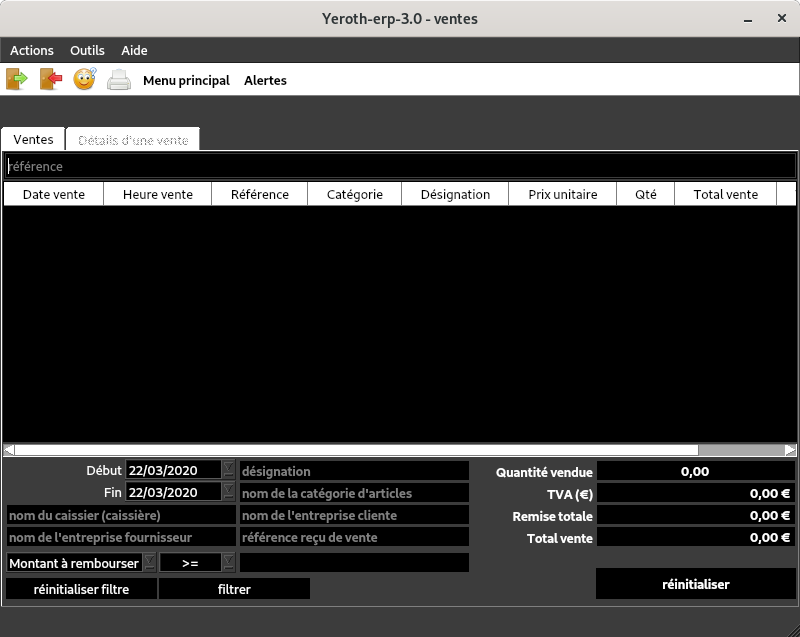
\includegraphics[scale=0.32]{../images/yeren-fenetre-caisse.png}
\caption{La fen\^etre des ventes}
\label{fig:fenetre-de-la-vente}
\end{figure}

\vspace{-1.9em}
\section{Les atouts de \yeren}
\vspace{-0.9em}
\begin{enumerate}[1)]
	\itemsep -0.3em
	\item une tr\`es grande stabilit\'e de l'application
	\item des utilisateurs avec des r\^oles (ou niveaux
	  d'acc\`es)
	\item un syst\`eme d'alerte qui comporte des alertes
	      sur des p\'eriodes de temps, et des alertes sur des
	      quantit\'es en stock
	\item la possibilit\'e de g\'en\'er\'er des factures au
	      petit format pour des imprimantes thermiques, ou bien
	      de g\'en\'er\'er des factures au format ''A4''
	\item Linux--Debian comme syst\`eme d'exploitation, car
	      tr\`es stable, performant, et moins vuln\'erable
	      aux attaques des pirates en comparaison aux autres
	      syst\`emes d'exploitation
	\item une interface ''ventes'' qui aide le \manager a
	      avoir une vue d'ensemble sur ses 
	      ventes~(voir la Figure~\ref{fig:fenetre-de-la-vente})
	\item une interface ''tableaux--de--bord'' qui
		  g\'en\`ere des diagrammes commerciaux au format PDF,
		  pour aider le \manager \`a prendre des d\'ecisions.
\end{enumerate}

\vspace{-1em}
\section{Le syst\`eme d'alerte}
\vspace{-0.5em}
\yeren permet \`a ses utilisateurs de cr\'eer
des alertes par rapport:
\begin{enumerate}[1)]
	\itemsep -0.5em
	\item \`a la quantit\'e restante d'un stock
	\item \`a une p\'eriode de temps bien
		d\'etermin\'ee (ceci aide pour les
		produits p\'erissables et pour les promotions).
\end{enumerate}

\vspace{-1em}

\subsection{Alertes sur une quantit\'e en stock}
\vspace{-0.1em}
Les utilisateurs ayant les r\^oles \administrateur ou
\manager peuvent cr\'eer des alertes qui se
d\'eclenchent lorsque la quantit\'e en stock d'un produit
atteint un certain nombre.

Par exemple Xavier (\manager) cr\'e une alerte sur le
produit ''mangue'' qui se d\'eclenche d\`es que sa quantit\'e
en stock atteint $100$; cette alerte est envoy\'ee et
accompagn\'ee d'un message \`a l'utilisateur Jean (\magasinier).

\vspace{-1em}

\subsection{Alertes sur une p\'eriode de temps}
\vspace{-0.1em}
Les utilisateurs ayant les r\^oles \magasinier ou
\manager peuvent cr\'eer des alertes qui se
d\'eclenchent d\`es qu'une date est atteinte.

Par exemple, un message d'alerte doit \^etre envoy\'e
a l'utilisateur Paul (\caissier) d\`es que
la date du 18 Novembre est atteinte afin que celui-ci
applique un rabais de $20\%$ sur chaque vente de
yaourt 'tr\`esbon' pendant une p\'eriode de 2 semaines.

\vspace{-1.1em}
\section{Le syst\`eme de gestion de base--de--donn\'ees}
\vspace{-0.9em}
\emph{MariaDB (MySQL)} est utilis\'e comme syst\`eme de gestion
de base de donn\'ees. \emph{MariaDB} est tr\`es stable,
performant, et gratuit.

\vspace{-1.1em}
\section{Le r\^ole \administrateur}\label{tachesadmin}
\vspace{-0.3em}
Parmi les t\^aches centrales du r\^ole \administrateur,
nous avons: \\
\{\emph{cr\'eer, modifier, lister, supprimer}\} $\longrightarrow$
\hspace{0.09cm} \{une alerte, une cat\'egorie de produit,
un compte client, un compte utilisateur, un compte
fournisseur, une localisation\}.

\vspace{-1em}
\section{Conclusion}
\vspace{-1em}
\begin{figure}[!htbp]
\centering
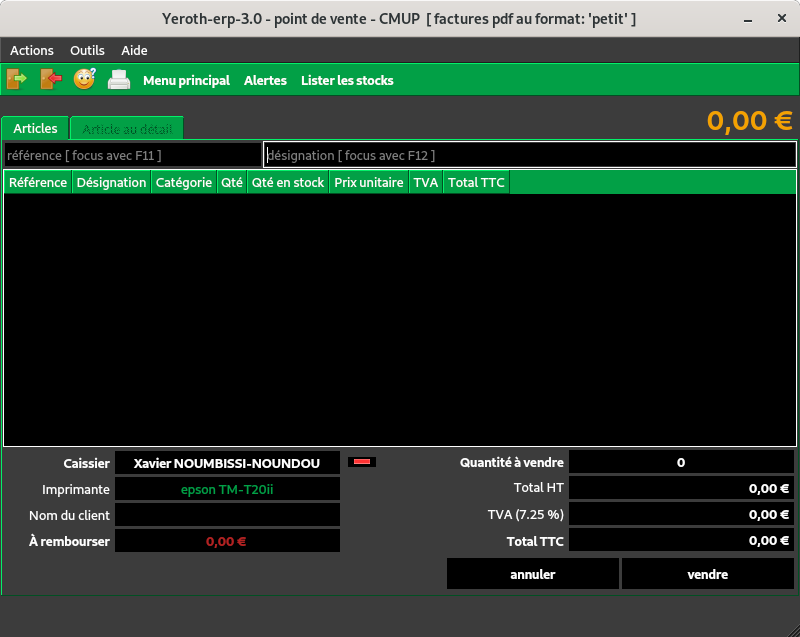
\includegraphics[scale=0.33]{../images/yeren-fenetre-caissier.png}
\caption{La fen\^etre de vente}
\label{fig:fenetre-de-vente}
\end{figure}

La Figure~\ref{fig:fenetre-de-vente} illustre la
fen\^etre pour faire les ventes d'articles.

\yeren ne fait pas de comptabilit\'e. \yeren est
disponible dans les langues Anglais et Fran\c{c}ais. 

\end{document}
